\label{CH6}

In this chapter, I analyse the effect of different ways of computing distributed representations of words, phrases and sentences on the downstream performance of~\emph{memory networks} REFs. Memory networks are one of relatively novel class of deeper neural network models that have been developed since 2014 and applied to language and reasoning problems [REFs]. These models are characterised not simply by their depth or quantity of internal representations, but by the explicit way in which they recruit information from those representations in order to complete their ultimate objective, by weighting them according to relevance. The component that computes the weights corresponding to each internal representation is typically referred to as an \emph{attention} mechanism. 

Neural networks with attention mechanisms are interesting for both scientific and engineering reasons. They can be understood as a rudimentary model of the poorly understood process of accessing and retrieving semantic memories in the human brain, a process that undoubtedly plays a critical part in human language understanding. Moreover, the attention mechanisms of trained networks can be interrogated to give a clear picture of which representations (and hence which information) is most relevant and useful to the network in the satisfaction of its objective, which can in turn facilitate a better understanding of the data and how networks can be modified to deliver improved performance.  

Various deep architectures with attention mechanisms were developed more or less simultaneously by different research groups [REFs]. The advantage of using memory networks for the present purpose is that, unlike the alternatives, the memory network setting makes a clear distinction between the various isolable components of the network, which themselves are defined very generally. It is therefore possible to focus on and and vary the component of interest (the module that represents text in semantic memory) while using neutral (weak prior) specifications of the other components. In this way, I hope to reach more robust conclusions about the effect of representational form on the network's objective task.  


\section{Testing representations `in the wild'}

Humans do not interpret language in isolation. The context in which words and sentences are understood, whether a conversation, book chapter or road sign, plays an important role in human comprehension \citep{altmann1988interaction,binder2011neurobiology}. In this work, I test the ability of neural language models (NLMs) to use such wider contexts to help make predictions about natural language. As I show, the way in which such contexts are represented is a critical factor in whether they can be exploited by the network.  

All of the analysis in this chapter is based on a new benchmark dataset (The Children's Book Test or CBT) designed to test the role of memory and context in language processing and understanding. The test requires models to make predictions about different types of missing words in children's books, given both nearby words and a wider context from the book. Humans taking the test predict all types of word with similar levels of accuracy. However, they rely on the wider context to make accurate predictions about named entities or nouns, whereas it is unimportant when predicting higher-frequency verbs or prepositions. 

As I show, state-of-the-art classical NLM architectures, Recurrent Neural Networks (RNNs) with Long-Short Term Memory (LSTMs), perform differently to humans on this task. They are excellent predictors of prepositions (\emph{on, at}) and verbs (\emph{run, eat}), but lag far behind humans when predicting nouns (\emph{ball, table}) or named entities (\emph{Elvis, France}). This is because their predictions are based almost exclusively on local contexts.  

In contrast, Memory Networks \citep{weston2014memory} are one of a class of `contextual models' that can interpret language at a given point in text conditioned directly on both local information and explicit representation of the wider context. As I show, on the CBT, Memory Networks can exploit contextual information to achieve markedly better prediction of named-entities and nouns than conventional language models. This is important for applications that require coherent semantic processing and/or language generation, since nouns and entities typically encode much of the important semantic information in language. 

However, not all contextual models reach this level of performance. The way in which wider context is represented in memory turns out be a critical factor in the network's ability to perform the task. Thus, analysis of the CBT with memory networks provides a useful benchmark for comparing the efficacy of different ways of representing words phrases and sentences (in the context). Moreover, unlike many of the evaluations used to evaluate representations in Chapters~\ref{CH2}-\ref{CH5}, this benchmark tests representations `in the wild': it measures the extent they enable a network trained on relatively downstream (or `extrinsic') language task to improve its performance. 

\section{The Children's Book Test}

The experiments in this paper are based on a new resource, the Children's Book Test, designed to measure directly how well language models can exploit wider linguistic context. The CBT is built from books that are freely available thanks to Project Gutenberg.\footnote{\url{https://www.gutenberg.org/}} Using children's books guarantees a clear narrative structure, which can make the role of context more salient. After allocating books to either training, validation or test setS, example `questions' (denoted \(x\)) are formed from chapters in the book by enumerating 21 consecutive sentences. 

In each question, the first 20 sentences form the \emph{context} (denoted \(S\)), and a word (denoted \(a\)) is removed from the 21$^{st}$ sentence, which becomes the \emph{query} (denoted \(q\)). Models must identify the \emph{answer word} \(a\) among a selection of 10 candidate answers (denoted \(C\)) appearing in the context sentences and the query. Thus, for a question answer pair  $(x,\, a)$: $x = (q,\,S,\,C)$; \(S\) is an ordered list of sentences; \(q\) is a sentence (an ordered list \(q=q_1 , \dots q_l\) of words) containing a missing word symbol; \(C\) is  a bag of unique words such that \(a \in C\),  its cardinality \(|C|\) is 10 and every candidate word \(w \in C\) is such that \(w \in q \cup S\). An example question is given in Figure~\ref{fig:goldilocks}.

\begin{figure}[h]
\centering
%\includegraphics[width=\textwidth]{qexample.pdf}
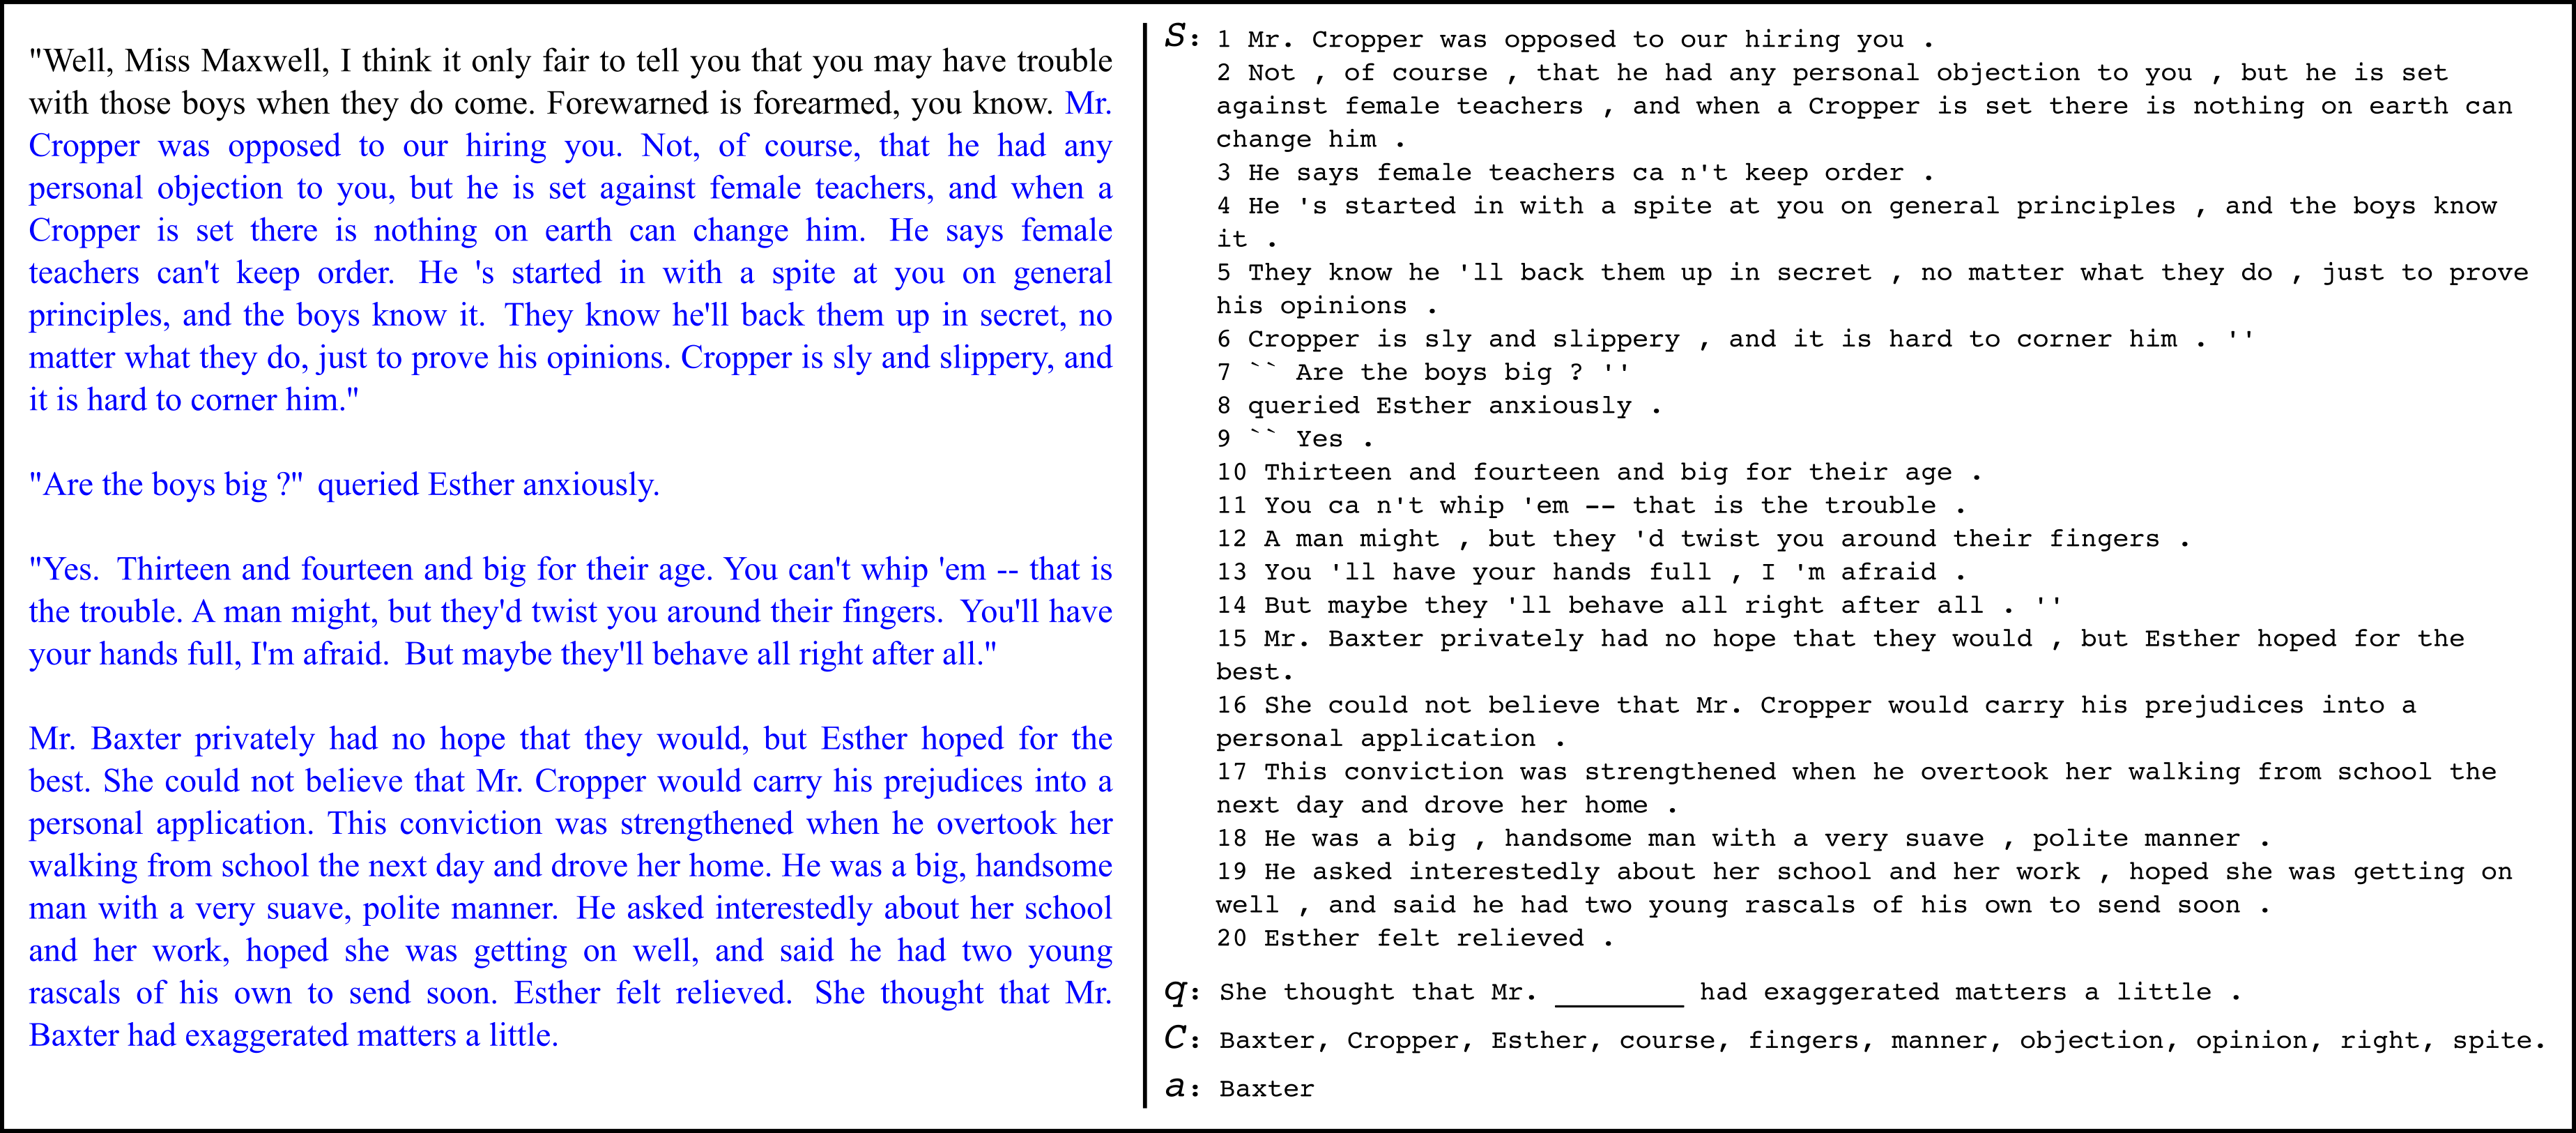
\includegraphics[width=\textwidth]{Chapter_6/cbt_fig1.png}
\caption{{\bf A Named Entity question from the CBT} (right), created from a book passage (left, in blue). In this case, the candidate answers \(C\) are both entities and common nouns, since fewer than ten named entities are found in the context.}
\label{fig:goldilocks}
\end{figure}

For finer-grained analyses, I created four classes of question by removing distinct types of word: Named Entities, (Common) Nouns, Verbs and Prepositions (based on output from the POS tagger and named-entity-recogniser in the Stanford Core NLP Toolkit \citep{manning2014stanford}). For a given question class, the nine incorrect candidates are selected at random from words in the context having the same type as the answer. The exact number of questions in the training, validation and test sets is shown in Table \ref{tab:cbt_stat}. Full details of the candidate selection algorithm (e.g. how candidates are selected if there are insufficient words of a given type in the context) can be found with the dataset.\footnote{The dataset can be downloaded from \url{http://fb.ai/babi/}.}

Classical language modelling evaluations are based on average perplexity across all words in a text. They therefore place proportionally more emphasis on accurate prediction of frequent words such as prepositions and articles than the less frequent words that transmit the bulk of the meaning in language \citep{baayen1996word}. In contrast, because the CBT allows focused analyses on semantic content-bearing words, it should be a better proxy for how well a language model can lend semantic coherence to applications including machine translation, dialogue and question-answering systems. 


\vspace{-2mm}
\begin{table}[ht]
\label{tab:cbt_stat}
  \begin{center}
    {\small 
      {\sc 
        \begin{tabular}{l|ccc}
          & Training & Validation & Test \\
          \hline
          \hline
          Number of books & 98 & 5 & 5 \\
          Number of questions (context+query)& 669,343 & 8,000 & 10,000  \\
          Average words in contexts & 465 & 435 & 445 \\
          Average words in queries & 31 & 27 & 29 \\
          Distinct candidates & 37,242 & 5,485 & 7,108 \\
          \hline
          Vocabulary size & \multicolumn{3}{|c}{53,628}\\
          \hline
        \end{tabular}
      }
    }
    \caption{\label{tab:cbt_stat} {\bf Statistics of the CBT.} Breakdown by question class is provided with the data set files.}
  \end{center}
\vspace*{-4ex}
\end{table}



%\begin{listenv}{An example question from the Named Entities section of the CBTest dataset, taken from The Jungle Book.} \itemsep1pt \parskip0pt \parsep0pt
%\tiny{
 % \item[C1] I will play with them again . ''
  %\item[C2]  `` Listen , man-cub , '' said the Bear , and his voice rumbled like thunder on a hot night .
  %\item[C3]   `` I have taught thee all the Law of the Jungle for all the peoples of the jungle -- except the Monkey-Folk who live in the trees .	
  %\item[C4]   They have no law .
  %\item[C5]   They are outcasts .
  %\item[C6]   They have no speech of their own , but use the stolen words which they overhear when they listen , and peep , and wait up above in the branches .
  %\item[C7]   Their way is not the way .
  %\item[C8]   They are without leaders .
  %\item[C9]   They have no remembrance .
  %\item[C10]   They boast and chatter and pretend that they are a great people about to do great affairs in the jungle , but the falling of a nut turns their minds to laughter and all is forgotten .
  %\item[C11]   I of the jungle have no dealings with them .
  %\item[C12]   I do not drink where the monkeys drink ; I do not go where the monkeys go ; I do not hunt where they hunt ; I do not die where they die .
  %\item[C13]   Hast thou ever heard me speak of the Bandar-log till today ? ''
  %\item[C14]   `` No , '' said Mowgli in a whisper , for the forest was very still now Baloo had finished .
  %\item[C15]   `` The Jungle-People put them out of their mouths and out of their minds .
  %\item[C16]   They are very many , evil , dirty , shameless , and they desire , if they have any fixed desire , to be noticed by the Jungle People .
  %\item[C17]   But I do not notice them even when they throw nuts and filth on the heads . ''
  %\item[C18]   He had hardly spoken when a shower of nuts and twigs spattered down through the branches ; and they could hear coughings and howlings and angry jumpings high up in the air among the thin branches.
  %\item[C19]   `` The Monkey-People are forbidden , '' said Baloo , `` forbidden to the Jungle-People ."
  %\item[C20]   Remember . 
  %\item[Query]   `` Forbidden , '' said Bagheera , `` but I still think \   \textunderscore\textunderscore\textunderscore\textunderscore\textunderscore\textunderscore \  should have warned thee against them ." 
  %\item[Answer]   Baloo 
  %\item[Candidates]    Bear|Bandar-log|Baloo|Jungle-People|Monkey-People|Mowgli|coughings|howlings|jumpings|man-cub
%}
%\end{listenv}
 

%\end{nonfloatlistenv}

\subsection{Related resources}
There are clear parallels between the CBT and the Microsoft Research Sentence Completion Challenge (MSRCC) \citep{zweig2011microsoft}, which is also based on Project Gutenberg (but not children's books, specifically). A fundamental difference is that, where examples in the MSRCC are made of a single sentence, each query in the CBT comes with a wider context. This tests the sensitivity of language models to semantic coherence beyond sentence boundaries. The CBT is also larger than the MRSCC (10,000 vs 1,040 test questions), requires models to select from more candidates on each question (10 vs 5), covers missing words of different (POS) types and contains large training and validation sets that match the form of the test set. 

There are also similarities between the CBT and the CNN/Daily Mail (CNN QA) dataset recently released by \cite{nips15_hermann}. This task requires models to identify missing entities from bullet-point summaries of online news articles. The CNN QA task therefore focuses more on paraphrasing parts of a text, rather than making inferences and predictions from contexts as in the CBT. It also differs in that all named entities in both questions and articles are anonymised so that models cannot apply knowledge that is not apparent from the article. I do not anonymise entities in the CBT, as I hope to incentivise models that can apply background knowledge and information from immediate and wider contexts to the language understanding problem.\footnote{See Appendix~\ref{ap:anon} for a sense of how anonymisation changes the CBT.} At the same time, the CBT can be used as a benchmark for general-purpose language models whose downstream application is semantically focused generation, prediction or correction. 
%
The CBT is also similar to the MCTest of machine comprehension \citep{richardson2013mctest}, in which children's stories written by annotators are accompanied by four multiple-choice questions. However, it is very difficult to train statistical models only on MCTest because its training set consists of only 300 examples.

\section{Studying memory representation with memory networks}

\label{sec:memnn}

Context sentences of $S$ are encoded into memories, denoted $m_i$, using a feature-map \(\phi(s)\) mapping sequences of words \(s \in S\) from the context to one-hot representations in \([0,1]^d\), where $d$ is typically the size of the word vocabulary. Memory networks are a comparatively new technology, and can be challenging to train as each constitutent component must be optimised via a single error signal backpropagated from the output predictions. Indeed, this work constitutes their first application to naturally occurring language. We therefore constrain our analyses to three simple (word-order independent) forms for forming representations \(s\) of the context, detailed below. Ultimately, however, as the infrastructure challenges reduce, the prior structures and representational forms for word, phrase or sentence representation treated in Chapters~\ref{CH2}-\ref{CH5} could also be used and might lead to improved results.

\begin{itemize}  %  [leftmargin=3mm]

\item {\bf Lexical memory:} Each word occupies a separate slot in the memory (each phrase \(s\) is a single word and \(\phi(s)\) has only one non-zero feature). To encode word order, time features are added as embeddings indicating the index of each memory, following \cite{sukhbaatar2015end}. 

\item {\bf Window memory:} Each phrase \(s\) corresponds to a window of text from the context $S$ centred on an individual mention of a candidate $c$ in $S$. Hence, memory slots are filled using windows of words \(\{ w_{i-(b-1)/2} \dots w_i \dots w_{i+(b-1)/2} \} \) where \(w_i\in C\) is an instance of one of the candidate words in the question.\footnote{See Appendix~\ref{ap:nonsparse-windows} for discussion and analysis of using candidates in window representations and training.} Note that the number of phrases \(s\) is typically greater than $|C|$ since candidates can occur multiple times in $S$. The window size \(b\) is tuned on the validation set. I experimented with encoding as a standard bag-of-words, or by having one dictionary per window position, where the latter performed best.

\item {\bf Sentential memory:} This setting follows the original implementation of Memory Networks for the bAbI tasks where the phrases \(s\) correspond to complete sentences of $S$.  For the CBT, this means that each question yields exactly 20 memories. I also use Positional Encoding (PE) as introduced by \cite{sukhbaatar2015end} to encode the word positions. 
\end{itemize}

The order of occurrence of memories is less important for sentential and window formats than for lexical memory. So, instead of using a full embedding for each time index, I simply use a scalar value which indicates the position in the passage, ranging from 1 to the number of memories. An additional parameter (tuned on the validation set) scales the importance of this feature. As I show in Appendix~\ref{ap:qa_cnn_ab_study}, time features only gave a marginal performance boost in those cases.

% In \citep{weston2014memory} the idea of attaching time features to memories is proposed so that the model is aware of which memories ``occur'' first, which was shown vital in some synthetic natural language tasks. Here, I implemented a very simple variant: each memory has an additional scalar feature ${\mbox{t}}(m')$ which indicates its position in the passage, ranging from 1 to the memory size. Scoring of a memory then becomes:
% \[
%    S_{time}(q, m') =  S(q, y) + \beta~ {\mbox{time}}(m')
% \]
% where an additional parameter $\beta$ (tuned on the validation set) indicates the importance of the time feature. However, as I will see in the experiments, this only gave a marginal performance boost on the tasks I consider in this paper.
% Note that, because time features are encoded in the memory (see below), this effectively models the memory as an ordered stream of individual words.  

For sentential and window memory formats, queries are encoded in a similar way to the memories: as a bag-of-words representation of the whole sentence and a window of size $b$ centred around the missing word position respectively.
%
For the lexical memory, memories are made of the $n$ words preceding the word to be predicted, whether these $n$ words come from the context or from the query, and the query embedding is set to a constant vector $0.1$. 

\subsection{End-to-end training} \label{sec:mod_o}

The {MemN2N} architecture, introduced by \cite{sukhbaatar2015end}, allows for a direct training of Memory Networks through backpropagation, and consists of two main steps.

First, `supporting memories', those useful to find the correct answer to the query $q$, are retrieved. This is done by embedding both the query and all memories into a single space of dimension $p$ using an embedding matrix $\bA\in\Re^{p \times d}$ yielding the query embedding  $\bq=\bA\phi(q)$ and memory embeddings $\{\bc_i=\bA\phi(s_i)\}_{i=1,\dots n}$, with $n$ the number of memories. %\footnote{To encode the position of words in the windows on the window memory setting, I used one embedding matrix per position, that is, $\bA$ is duplicated $b$ times.} 
%
\if0 %old stuff
The match between $\bq$ and each memory $\bc_i$ in the embedding space is fed through a softmax layer giving a distribution \(\{\alpha_i\}_{i=1, \dots n}\) of matching scores defined by $\alpha_i =  e^{\bc_i^\top\bq} / \sum_j e^{\bc_j^\top\bq}$. These weights are used to return a weighted average of memories as the first supporting memory:\footnote{Such a weighted average over memories can also be understood as the model's \emph{attention} mechanism.} 
\begin{equation} \label{eq:eq_o}
  \bm_{o1} = \sum_{i=1 \dots n} \alpha_{i} \bm_i \,,
\end{equation}
\fi
The match between $\bq$ and each memory $\bc_i$ in the embedding space is fed through a softmax layer giving a distribution \(\{\alpha_i\}_{i=1, \dots n}\) of matching scores which are used as an \emph{attention} mechanism over the memories to return the first supporting memory:%\footnote{Such a weighted average over memories can also be understood as.} 
\begin{equation} \label{eq:eq_o}
  \bm_{o1} = \sum_{i=1 \dots n} \alpha_{i} \bm_i\,, \mbox{~~~~~~}\text{with~~~~~}\alpha_i =  \frac{e^{\bc_i^\top\bq}}{\sum_j e^{\bc_j^\top\bq}}, \, i=1,\dots n,
\end{equation}
and where $\{\bm_i\}_{i=1,\dots n}$ is a set of memory embeddings obtained in the same way as the $\bc_i$, but using another embedding matrix $\bB\in\Re^{p\times d}$.

%The scoring function \(S_O \) is an embedding model of the form \[ S_o(q,y) = \phi_q(q)^\top U_o^\top U_o \phi_y(y)\] parameterised by weight matrix \(U_o\).

During training, optimization is carried out using stochastic gradient descent (SGD). Extra experimental details and hyperparameters are given in Appendix~\ref{ap:hp}.

%\todo{something about multi-core training: AB: not sure especially since word-memnn run on GPU. seems to complexify for nothing.}. 


\subsection{Self-supervision for Window Memories} \label{sec:ssup}

%The softmax operation over memories in eq~\eqref{eq:eq_o} of the ${\bf O}$ module can dilute information across the whole context in cases where a single memory is enough to answer correctly. 

Training a memory network with multiple components by backpropagating a single error signal derived from its final predictions can constitute a challenging non-convex optimisation problem. After initial experiments, I found that it was beneficial to use a heuristic to provide a stronger signal for learning memory access. A related approach was successfully applied by \cite{bordes2015large} to question answering about knowledge bases.

\if0
In a `self-supervised' Memory Network, a heuristic informs the network which memories to attend to for each training question. Intuitively, this can help to overcome the difficult optimization inherent in training a single network jointly to access information and use it effectively. For the CBT, the heuristic identifies potentially correct memories as those whose corresponding candidate is the correct answer. In the common case where more than one memory contains the correct answer, the heuristic picks the single memory $\tilde{m}$ that is scored highest by the query in the embedding space defined by $\bA$.\footnote{TF-IDF similarity worked almost as well in the experiments, but a random choice over positives did not.} The model incorporates this information by taking a gradient step using SGD to force its memory retrieval network, for each example, to give a higher score to the supporting memory $\tilde{m}$ than other memories.
\fi

		
Memory supervision (knowing which memories to attend to) is not provided at training time but is inferred automatically using a simple heuristic: during training, the correct supporting memory is assumed to be among the window memories whose corresponding candidate is the correct answer.		
%		
In the common case where more than one memory contains the correct answer, the model picks the single memory $\tilde{m}$ that is already scored highest by itself, i.e. scored highest by the query in the embedding space defined by $\bA$.\footnote{TF-IDF similarity worked almost as well in the experiments, but a random choice over positives did not.} 

Training is carried out by making gradient steps using SGD to force the model, for each example, to give a higher score to the supporting memory $\tilde{m}$ relative to any other memory from any other candidate.
%
Instead of using  eq~\eqref{eq:eq_o}, the model selects its top relevant memory using:
\begin{equation} \label{eq:salient}
  m_{o1} = \argmax_{i=1,\dots n} \bc_i^\top\bq \, .%\footnote{This hard selection was actually used in the original Memory Network paper \citep{weston2014memory}}
\end{equation}
%
If $m_{o1}$ happens to be different from $\tilde{m}$, then the model is updated.


%

%


%
At test time, rather than use a hard selection as in eq~\eqref{eq:salient}
the model scores each candidate not only with its highest scoring memory
but with the sum of the scores of all its corresponding windows after passing all scores through a softmax. That is, the score of a candidate is defined by the sum of the $\alpha_i$ (as used in eq~\eqref{eq:eq_o}) of the windows it appears in. This relaxes the effects of the \(max\) operation and allows for all windows associated with a candidate to contribute some information about that candidate. As shown in the ablation study in Appendix~\ref{ap:qa_cnn_ab_study}, this results in slightly better performance on the CNN QA benchmark compared to hard selection at test time.

Note that self-supervised Memory Networks do not exploit any new label information beyond the training data. % (compared to e.g. the strong supervision in the bAbI tasks of \cite{}).
The approach can be understood as a way of achieving \emph{hard attention} over memories, to contrast with the \emph{soft attention}-style selection described in Section~\ref{sec:mod_o}. Hard attention yields significant improvements in image captioning \citep{xu2015show}. However, where \cite{xu2015show} use the REINFORCE algorithm \citep{williams1992simple} to train through the max of eq~\eqref{eq:salient}, the self-supervision heuristic permits direct backpropagation.


% In the common case where more than one memory contains the correct answer, I select the favored memory using one of two strategies:
% \begin{itemize}
% \item[(i)] Select the memory containing the correct answer that also has the with highest TFDIF bag-of-words score with the query as the supervised target.
% \item[(ii)] Use the model itself selects the highest scoring of all memories that contain the correct answer. 
% \end{itemize}
% Both approaches end up working quite well in the experiments. 

%\todo{I am a little concerned this paragraph seems to contradict the first paragraph in this section   "The softmax operation....". What do you think?}


% One can thus instead consider the scoring function:
% \[
% a = \argmax_{w \in W}\{ S_R(q,w) + S_R(\textbf{m}_1,w)
%   + \alpha \sum_{k : y(m_k) = y(m_1)} S_R(\textbf{m}_k,w)  \}
% \]
% where $y(m')$ is the label (output candidate word) for the memory $m'$. Note that this approach is only viable for the window memory approach where each memory is associated with an explicit candidate. This gives one more parameter, $\alpha$, to be learnt.

\section{Baseline and ocmparison models}


In addition to memory network variants, I also applied many different types of
 language modelling and machine reading architectures to the CBT.
%To place the performance of different Memory Network designs in context, I also applied 
%various existing language modelling and machine reading architectures to the CBT.

\subsection{Non-learning baselines}
I implemented two simple baselines based on word frequencies. For the first, I selected the most frequent candidate in the entire training corpus. In the second, for a given question I selected the most frequent candidate in its context. In both cases I broke ties with a random choice. 

I also tried two more sophisticated ways to rank the candidates that do not require any learning on the training data. The first is the `sliding window' baseline applied to the MCTest by \cite{richardson2013mctest}. In this method, ten `windows' of the query concatenated with each possible candidate are slid across the context word-by-word, overlapping with a different subsequence at each position. The overlap score at a given position is simply word-overlap weighted TFIDF-style based on frequencies in the context (to emphasize less frequent words). The chosen candidate corresponds to the window that achieves the maximum single overlap score for any position. Ties are broken randomly. 

The second method is the word distance benchmark applied by \cite{nips15_hermann}. For a given instance of a candidate \(w_i\) in the context, the query \(q\) is `superimposed' on the context so that the missing word lines up with \(w_i\), defining a subsequence \(s\) of the context. For each word \(q_i\) in \(q\), an alignment penalty $P = \min( \min_{j = 1 \dots |s|} \{|i - j| : s_j = q_i\}, m)$ is incurred. The model predicts the candidate with the instance in the context that incurs the lowest alignment penalty. I tuned the maximum single penalty \(m=5\)  on the validation data.  

\subsection{N-gram language models}
I trained an n-gram language model using the KenLM toolkit \citep{Heafield-estimate}. I used Knesser-Ney smoothing, and a window size of 5, which performed best on the validation set.
%
I also compare with a variant of language model with cache \citep{kuhn1990cache}, where I linearly interpolate the n-gram model probabilities with unigram probabilities computed on the context.

\subsection{Supervised embedding models}
To directly test how much of the CBT can be resolved by good quality dense representations of words (word embeddings), I implement a supervised embedding model similar to that of \citep{weston2010large}. In these models I learn both input and output embedding matrices \(\bA,\,\bB \in \Re^{p\times d}\) for each word in the vocabulary ($p$ is still the embedding dimension and $d$ the vocabulary size). For a given input passage \(q\) and possible answer word \(w\), the score is computed as \(S(q,\,w) = \phi(q) \bA ^\top \bB \phi(w) \), with \(\phi\) the feature function defined in Section~\ref{sec:memnn}.
These models can be considered as lobotomised Memory Networks with zero hops, 
i.e. the attention over the memory component is removed.

I encode various parts of the question as the input passage: the entire {\bf context + query}, just the {\bf query}, a sub-sequence of the query defined by a {\bf window} of maximum \(b\) words centred around the missing word, and a version ({\bf window + position}) in which I use a different embedding matrix  for encoding each position of the window. I tune the window-size \(d=5\) on the validation set. 


\subsection{Recurrent language models}
I trained probabilistic RNN language models with LSTM activation units on the training stories (5.5M words of text) using minibatch SGD to maximise the negative log-likelihood of the next word. Hyper-parameters were tuned on the validation set. The best model had both hidden layer and word embeddings of dimension $512$.
%
When answering the questions in the CBT, I allow one variant of this model ({\bf context + query}) to `burn in' by reading the entire context followed by the query and another version to read only the {\bf query} itself (and thus have no access to the context). Unlike the canonical language-modelling task, all models have access to the query words {\em after} the missing word (i.e if $k$ is the position of the missing word, I rank candidate \(c\) based on \(p(q_1 \dots q_{k-1}, c , q_{k+1} \dots q_l)\) rather than simply \(p(q_1 \dots q_{k-1},c)\)).

\cite{mikolov2012context} previously observed performance boosts for recurrent language models by adding the capacity to jointly learn a document-level representation. I similarly apply a context-based recurrent model to the language-modelling tasks, but opt for the convolutional representation of the context applied by \cite{rush2015neural} for summarisation. the Contextual LSTM (CLSTM) learns a convolutional attention over windows of the context given the objective of predicting all words in the query. I tuned the window size (\(w=5\)) on the validation set. As with the standard LSTM, I trained the CLSTM on the running-text of the CBT training set (rather than the structured query and context format used with the Memory Networks) since this proved much more effective, and I  report results in the best setting for each method.

\subsection{Human performance}

I recruited 15 native English speakers to attempt a randomly-selected 10\% from each question type of the CBT, in two modes either with question only or with question+context (shown to different annotators), giving 2000 answers in total.
 % so that each annotator answered $\approx$ 132 questions. 
To the knowledge, this is the first time human performance has been quantified on a language modelling task based on %multiple participants and 
different word types and context lengths.

%As a result, I do not have a measure of the variance of the human judgements but I have a better coverage of questions, which was the priority.

\subsection{Other related approaches}
The idea of conditioning language models on extra-sentential context is not new. Access to document-level features can improve both classical language models \citep{mikolov2012context} and word embeddings \citep{huang2012improving}. Unlike the present work, these studies did not explore different representation strategies for the wider context or their effect on interpreting and predicting specific word types.

The original Memory Networks \citep{weston2014memory} used hard memory selection with additional labeled supervision for the memory access component, and
%used self-supervised memory access and were 
were applied to question-answering tasks 
%in which language was generated to describe the content of 
over knowledge bases or simulated worlds. \cite{sukhbaatar2015end} and \cite{kumar2015ask} trained Memory Networks with RNN components end-to-end with soft memory access, and applied them to additional language tasks. The attention-based reading models of \cite{nips15_hermann} also have many commonalities with Memory Networks, differing in word representation choices 
and attention procedures.
%I guess I don't want to emphasize this so much if it doesnt work: %, one key difference being the absence of iterative access, based on the entire query, to the memory-like representations.
Both \cite{kumar2015ask} and \cite{nips15_hermann} propose bidirectional RNNs as a way of representing previously read text. the experiments in Section~\ref{sec:results} provide a possible explanation for why this is an effective strategy for semantically-focused language processing: bidirectional RNNs naturally focus on small windows of text in similar way to window-based Memory Networks. 

Other recent papers have proposed RNN-like architectures with new ways of reading, storing and updating information to improve their capacity to learn algorithmic or syntactic patterns \citep{joulin2015inferring,dyer2015transition,grefenstette2015learning}. While I do not study these models in the present work, the CBT would be ideally suited for testing this class of model on semantically-focused language modelling.  

\section{Results}


\label{sec:results}

\begin{table}[t]
\newcommand{\mc}[1]{\multicolumn{1}{l|}{#1}}
  \begin{center}
    \resizebox{1\linewidth}{!}{
      {\sc 
        \begin{tabular}{l|cccc}
          \mc{Methods} & Named Entities & Common Nouns & Verbs & Prepositions
          \\
          \hline
          \hline
          \mc{Humans (query)$^{(*)}$} & 0.520 & 0.644 & 0.716 & 0.676 \\
          \mc{Humans (context+query)$^{(*)}$} &{\it \textbf{0.816}} & {\it \textbf{ 0.816}} & {\it \textbf{0.828}} & 0.708 \\
          \hline 
          \hline 
          \mc{Maximum frequency (corpus)} & 0.120 & 0.158 & 0.373 & 0.315 \\
          \mc{Maximum frequency (context)} & 0.335 & 0.281 & 0.285 & 0.275 \\
          \mc{Sliding window} & 0.168 & 0.196 & 0.182 & 0.101 \\
          \mc{Word distance model} & 0.398 & 0.364 & 0.380 & 0.237 \\
          \mc{Kneser-Ney language model} & 0.390 & 0.544 & 0.778 & 0.768 \\                                                                    
          \mc{Kneser-Ney language model + cache} & 0.439 & 0.577 & 0.772 & 0.679 \\ 
          \hline
          \mc{\starspace (context+query)} & 0.253 & 0.259 & 0.421 & 0.315 \\
          \mc{\starspace (query)} & 0.351 & 0.400 & 0.614 & 0.535 \\
          \mc{\starspace (window)} & 0.362 & 0.415 & 0.637 & 0.589 \\
          \mc{\starspace (window+position)} & 0.402 & 0.506 & 0.736 & 0.670 \\
          \hline 
          \mc{LSTMs (query)} & 0.408 & 0.541 & 0.813 & 0.802 \\
          \mc{LSTMs (context+query)} & 0.418 & 0.560 & \bf 0.818 & 0.791 \\
          \mc{Contextual LSTMs (window context)} & 0.436 & 0.582 & 0.805 & \bf 0.806\\
          \hline
          \hline
          MemNNs  (lexical memory) &   0.431 & 0.562 & 0.798 & 0.764 \\
          MemNNs  (window memory) &  0.493 & 0.554 & 0.692 & 0.674 \\
          MemNNs  (sentential memory + PE) & 0.318 & 0.305 & 0.502 & 0.326 \\
          MemNNs  (window memory + self-sup.) & \bf 0.666 & \bf 0.630 & 0.690 & 0.703\\
          \hline 
          %MemNNs  (window + self-sup. + anonym.) & 0.581 & 0.473 & 0.474 & 0.522\\
          %\hline
        \end{tabular}
      }
    }
    \caption{\label{tab:cbt_res} {\bf Results on CBT test set.} $^{(*)}$Human results were
      collected on 10\% of the test set.}\label{tab:cbt_res}
  \end{center}
  \vspace*{-4ex}
\end{table}



\paragraph{Modelling syntactic flow} 
In general, there is a clear difference in model performance according
to the type of word to be predicted. the main results in Table \ref{tab:cbt_res}
%As can be seen in Table
%\ref{tab:cbt_res}, conventional language models are very good at
show  conventional language models are very good at
predicting prepositions and verbs, but less good at predicting named
entities and nouns. Among these language models, and in keeping with
established results, RNNs with LSTMs demonstrate a small gain on
n-gram models across the board, except for named entities where the cache is beneficial. 
In fact, LSTM models are better than humans at predicting prepositions, which suggests that there are cases in which several of the candidate prepositions are `correct', but annotators prefer the less frequent one.  Even more surprisingly, when only local context (the query) is available, both LSTMs and n-gram models predict verbs more accurately than humans. This may be because the models are better attuned to the distribution of verbs in children's books, whereas humans are unhelpfully influenced by their wider knowledge of all language styles.\footnote{I did not require the human annotators warm up by reading the 98 novels in the training data, but this might have led to a fairer comparison.} When access to the full context is available, humans do predict verbs with slightly greater accuracy than RNNs. 

\paragraph{Capturing semantic coherence} The best performing Memory
Networks predict common nouns and named entities more
accurately than conventional language models. Clearly, in doing so,
these models rely on access to the wider context (the
supervised {\small \sc{embedding model (query)}}, which is equivalent to the
memory network but with no contextual memory, performs poorly in this
regard). The fact that LSTMs without attention perform similarly on
nouns and named entities whether or not the context is available
confirms that they do not effectively exploit this context. This may
be a symptom of the difficulty of storing and retaining information
across large numbers of time steps that has been previously observed
in recurrent networks (See e.g. \cite{bengio1994learning}). 
%LSTMs have been shown to do well
%on tasks such as 
%translation between close languages \cite{sutskever2014sequence} but note that only consists of a single source sentence.

%LSTMs are able to overcome this issue for related problems such as translation between close languages \cite{sutskever2014sequence}. The reason that they cannot in the present case may be due to the low frequency of nouns and entities and the nature of the missing word prediction task, which together make it challenging for the multiple memory gates to learn information retention strategies that effectively generalise to the test set. 


\paragraph{Getting memory representations `just right'} Not all memory
networks exploited the context to achieve
decent prediction of nouns and named entities.
For instance, when each sentence in the context is stored as an ordered sequence of word
embeddings (\emph{sentence mem + PE}), performance is quite
poor in general. Encoding the context as an unbroken sequence of individual
words (\emph{lexical memory}) works well for capturing prepositions
and verbs, but is less effective with nouns and entities. In contrast,
\emph{window memories} centred around the
candidate words are more useful than either word-level or
sentence-level memories when predicting named entities and nouns. 



%
%This is confirmed by the strong performance of the CLSTM implementation,
%which also relies on attention over window-like representations of the context.
% indicate the great fit of
%this format for this task.

\begin{figure}[ht]
\newcommand{\mc}[1]{\multicolumn{2}{l}{#1}}
  \begin{center}
   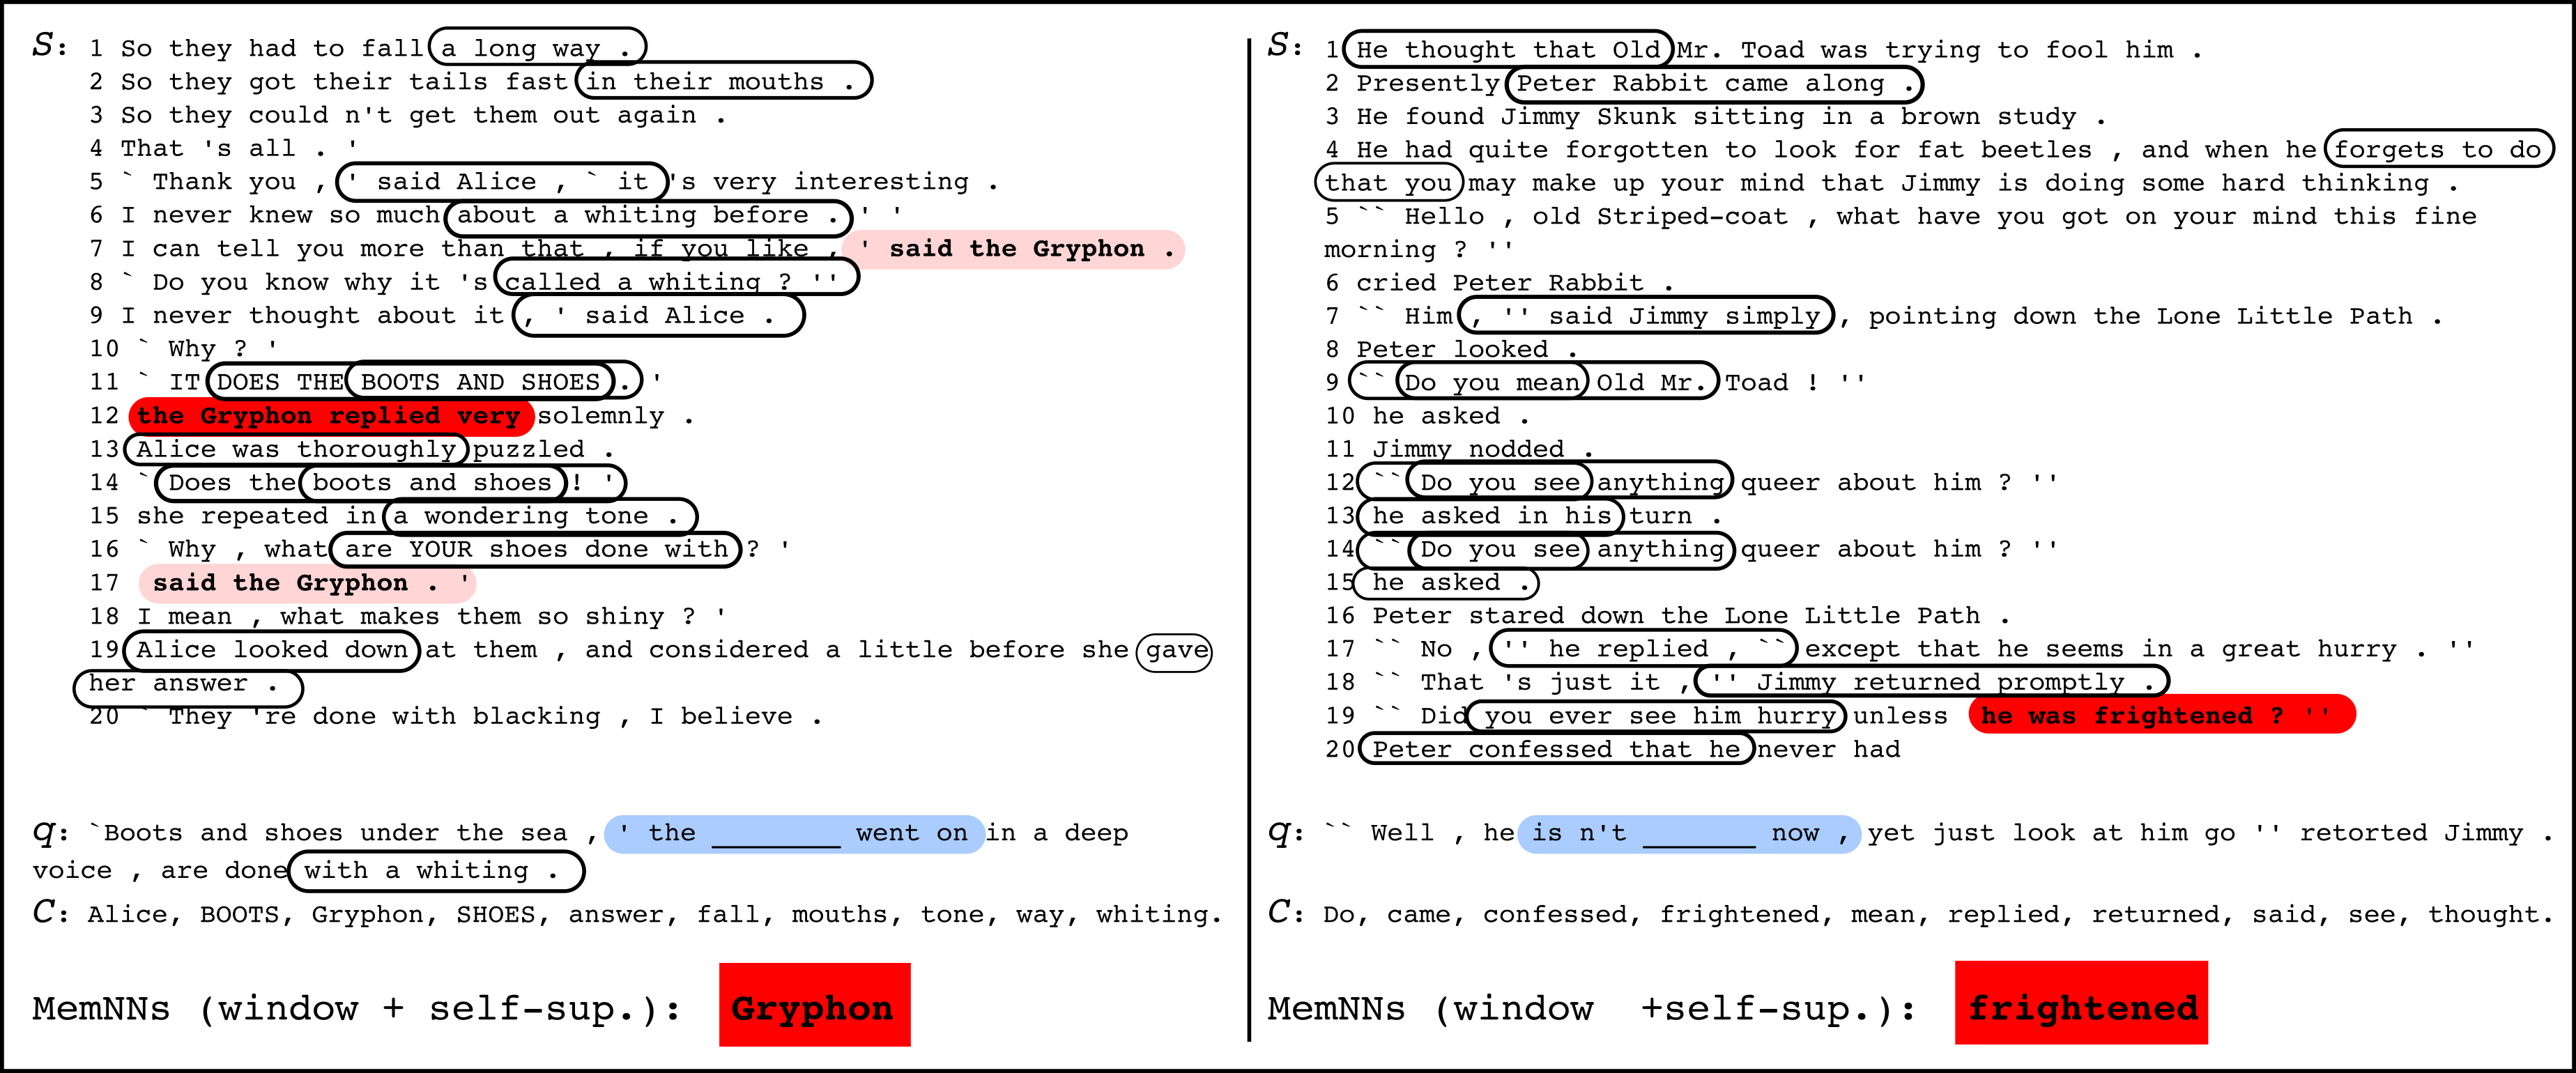
\includegraphics[width=\textwidth]{Chapter_6/cbt_fig2.png}
      \caption{\label{tab:ex_pred_cbt} {\bf Correct predictions of
          MemNNs (window memory + self-supervision) on CBT} on Named Entity (left) and
          Verb (right). Circled phrases indicate all considered
          windows; red ones are the ones corresponding to the returned
          (correct) answer; the blue windows represent the queries.}\label{tab:ex_pred_cbt}
    \end{center}
  \vspace*{-2ex}
\end{figure}


\paragraph{Self-supervised memory retrieval} 
%
The window-based Memory Network with self-supervision (in which a hard attention selection 
is made among window memories during training)
outperforms all others at predicting named entities and common nouns.
%
%Examples of predictions of this model for two CBT questions are shown in Figure~\ref{tab:ex_pred_cbt}. 
%
Examples of predictions made by this model for two CBT questions are shown
in Figure~\ref{tab:ex_pred_cbt}. It is notable that this model is able to achieve the strongest performance with only a simple window-based strategy for representing questions. 
%\
%Yet, this simpler model outperforms all other more
%sophisticated approaches at predicting the most semantically
%informative words because it captures conveniently word neighborhoods
%and can be trained efficiently.
%

% \footnote{The rather low performance of humans on prepositions might
% also be due to the particular syntax involved in the books of CBT,
% mostly published in late 19th - early 20th century.}


\if0
\begin{figure}[ht]
\newcommand{\mc}[1]{\multicolumn{2}{l}{#1}}
  \begin{center}
    \resizebox{0.8\linewidth}{!}{
      \begin{tabular}{|l|l|}
        % 1 & So they had to fall a long way.	\\
        % 2 & So they got their tails fast in their mouths.	\\
        % 3 & So they couldn't get them out again.	\\
        % 4 & That's all. '\\
        % 5 & ` Thank you, ' said Alice, ` it's very interesting.\\
        % 6 & I never knew so much about a whiting before. '\\	
        $\cdots$ & $\cdots$ \\
        7 & ` I can tell you more than that, if you like, ' said the Gryphon.\\
        8 & ` Do you know why it's called a whiting? '\\	
        9 & ` I never thought about it, ' said Alice .\\
        10 & ` Why? '	\\
        11 & ` IT DOES THE BOOTS AND SHOES. '	\\
        12 & \textbf{the Gryphon replied very} solemnly.	\\
        13 & Alice was thoroughly puzzled.	\\
        14 & ` Does the boots and shoes! '	\\
        15 & she repeated in a wondering tone.	\\
        16 & ` Why , what are YOUR shoes done with? '	\\
        17 & said the Gryphon.	\\
        18 & ` I mean , what makes them so shiny? '	\\
        19 & Alice looked down at them , and considered a little before she gave her answer.	\\
        20 & ` They're done with blacking, I believe. '	\\
        \mc{{\sc Query}: ` Boots and shoes under the sea, ' the \underline{\mbox{~~~~~~~~}} went on in a deep voice , ` are done with a whiting.'} \\
        \hline
        \mc{{\sc Candidates}: Alice, boots, Gryphon, shoes, answer, fall, mouths, tone, way, whiting}\\
        \hline
        \mc{{\sc MemNNs (salient memory)}: {\bf Gryphon}}\\
        \hline
      \end{tabular}
      }
      \caption{\label{tab:ex_pred_cbt} {\bf Example of prediction of MemNNs (salient memory) on CBT.} The bold phrase in sentence 12 is the selected relevant convolutional memory. }\label{tab:ex_pred_cbt}
    \end{center}
  \vspace*{-2ex}
\end{figure}
\fi
	




\begin{table}[ht]
  \begin{center}
   \label{tab:qacnn_res}
    \resizebox{1\linewidth}{!}{
%    {\small
      {\sc 
        \begin{tabular}{l|cc}
          Methods & Validation & Test \\
          \hline
          \hline
          Maximum frequency (article)$^{(*)}$ & 0.305 & 0.332 \\
          Sliding window & 0.005 & 0.006 \\
          Word distance model$^{(*)}$ & 0.505 & 0.509 \\
          \hline 
          Deep LSTMs (article+query)$^{(*)}$ & 0.550 & 0.570 \\
          Contextual LSTMs (``Attentive reader'')$^{(*)}$ & 0.616 & 0.630 \\
          Contextual LSTMs (``Impatient reader'')$^{(*)}$ & 0.618 & 0.638 \\
          \hline
%          MemNNs (lexical memory) & & \\
          MemNNs (window memory) & 0.580 & 0.606 \\
          MemNNs (window memory + self-sup.) & 0.634 & 0.668 \\
          \hline
          MemNNs (window memory + ensemble) & 0.612 & 0.638 \\ 
          MemNNs (window memory + self-sup.  + ensemble) & 0.649 & 0.684 \\
          \hline
          MemNNs (window  + self-sup.  +  ensemble + exclud. coocurrences) & \bf 0.662 & \bf 0.694 \\
          \hline
        \end{tabular}
      }
    }
    \caption{\label{tab:qacnn_res} {\bf Results on CNN QA.} $^{(*)}$Results taken from \cite{nips15_hermann}.}\label{cnn}
  \end{center}
  \vspace*{-2ex}
\end{table}


\subsection{News Article Question Answering}
To examine how well the conclusions generalise to different machine
reading tasks and language styles, I also tested the
best-performing Memory Networks on the CNN QA task \citep{nips15_hermann}.\footnote{The CNN QA dataset was released after the primary experiments were completed, hence I experiment only with one of the two large datasets released with that paper.} This dataset consists of 93k news articles from the CNN website, each coupled with a question derived from a bullet point summary accompanying the article, and a single-word answer. The answer is always a named entity, and all named entities in the article function as possible candidate answers.

As shown in Table~\ref{cnn}, the window model without self-supervision 
achieves similar
performance to the best approach proposed for the task by \cite{nips15_hermann}
when using an ensemble of MemNN models.
the use of an ensemble 
is an alternative way of replicating the application of \emph{dropout}~\citep{hinton2012improving} in the previous best
approaches \citep{nips15_hermann} as ensemble averaging has similar effects to dropout~\citep{wan2013regularization}.
When self-supervision is added, the Memory Network
greatly surpasses the state-of-the-art on this task. 
Finally, the last line of
Table~\ref{cnn} (\emph{excluding co-occurrences}) shows how an additional heuristic, removing from the candidate list all named entities
already appearing in the bullet point summary, boosts performance even further.


Some common principles may explain the strong
performance of the best performing models on this
task. The attentive/impatient reading models encode the articles using bidirectional RNNs
\citep{graves2008unconstrained}. For each word in
the article, the combined hidden state of such an RNN naturally
focuses on a window-like chunk of surrounding text, much like the window-based memory network or the CLSTM. Together, these results therefore support the principle that the most informative representations of text correspond to sub-sentential chunks. Indeed, the observation that the most informative representations
for neural language models correspond to small chunks of text is
also consistent with recent work on neural machine translation, in which
\cite{luong2015effective} demonstrated improved performance by
restricting their attention mechanism to small  windows of
the source sentence.


Given these commonalities in how the reading models and Memory
Networks represent context, the advantage of the best-performing
Memory Network instead seems to stem from how it accesses or retrieves
this information; in particular, the hard attention and
self-supervision. Jointly learning to access and use information is a
difficult optimization. Self-supervision in particular makes effective
Memory Network learning more tractable.\footnote{See the appendix for an ablation study in which optional features of the memory network are removed.} 

\section{Conclusion}

TO DO

MAKE IT MORE ABOUT MEMORY REPRESENTATION, LESS ABOUT CBT AND MEMNNs

I have presented the Children's Book Test, a new semantic language modelling benchmark. The CBT measures how well models can use both local and wider contextual information to make predictions about different types of words in children's stories. By separating the prediction of syntactic function words from more semantically informative terms, the CBT provides a robust proxy for how much language models can impact applications requiring a focus on semantic coherence. 

I tested a wide range of models on the CBT, each with different ways of
representing and retaining previously seen content. This enabled us to draw novel insights into the optimal strategies for representing and accessing semantic information in memory. One consistent finding was that memories that encode sub-sentential chunks (windows) of informative text 
seem to be most useful to neural nets when interpreting and modelling language. 
However, the results indicate that the
most useful text chunk size depends on the modeling task 
(e.g. semantic content vs. syntactic function words).
%One should be careful in how explicit 
%memories are defined since the best choice might depend on the task at 
%hand: on the CBT, windows are optimal, but on the
%bAbI tasks, sentences have shown to be adequate.
% 
I showed that Memory Networks that adhere to this principle can be efficiently trained using a simple
self-supervision to surpass all other methods for predicting named
entities on both the CBT and the CNN QA
benchmark, an independent test of machine reading. 
%


